\subsection{Алгоритм перетворення даних в граф}
\label{subsec:models-to-graph}

Щоб забезпечити ефективне планування маршрутів і навігацію в транспортній системі, моделі даних, що представляють станції, маршрути, пересадки і пункти призначення, повинні бути перетворені в графову структуру. Таке графове представлення дозволяє застосовувати різні графові алгоритми, такі як алгоритм Дейкстри або алгоритм Єна, для пошуку найкоротших маршрутів і оптимізації навігації.

Перетворення починається з того, що кожна станція(представлена моделлю "Station") розглядається як вершина графа. Унікальні ідентифікатори станцій, такі як їхні ідентифікатори, можуть бути використані як ідентифікатори для відповідних вузлів.

З'єднання між станціями представлені моделлю "Waypoint", відображаються у вигляді ребер на графі. Кожне ребро представляє прямий зв'язок між двома станціями, використовуючи час подорожі між ними як вагу ребра. Атрибути з'єднання, такі як ідентифікатор станції відправлення, ідентифікатор станції призначення, час подорожі, розклад відправлення, пов'язані з відповідним ребром, потрібно зберігати, щоб використовувати ці дані в подальшій обробці.

Крім того, маршрутні точки, пов'язані з кожним маршрутом, слугують проміжними пунктами на маршруті. Ці точки можуть бути представлені у вигляді вузлів на графі і з'єднані з відповідними станціями ребрами. Таке включення маршрутних точок підвищує точність і гнучкість планування маршруту, дозволяючи здійснювати більш точну навігацію.

Після перетворення моделей у графове представлення можна застосовувати широкий спектр графових алгоритмів для пошуку найкоротших маршрутів, врахування розкладів та оптимізації навігації на основі певних критеріїв. Графова структура забезпечує потужну та гнучку основу для планування маршрутів у транспортній системі, забезпечуючи ефективну та надійну навігацію для користувачів.

\begin{figure}[!h]
    \centering
    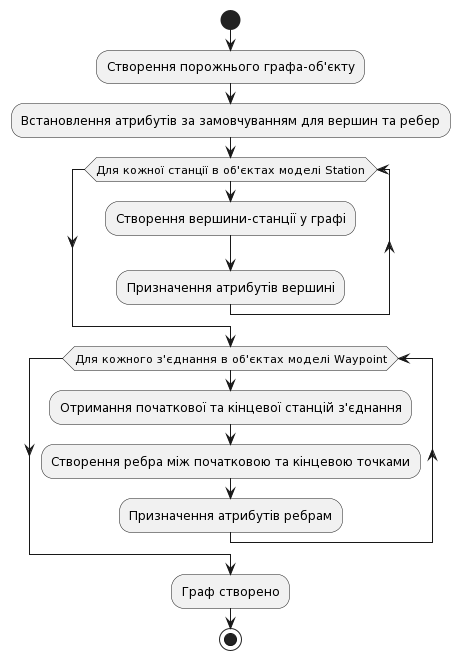
\includegraphics[scale=0.6]{content/chapters/2-implementation-methods/assets/img/models-to-graph_diagram.png}
    \caption{Діаграма описаних моделей}
    \label{fig:bfs}
\end{figure}